\section{System Design}
% 
//Chapter introduction to be written

There are several possibilities, one wants to exchange cryptocurrency on the internet. Let's consider, that Alice wants to exchange Bitcoin for Ether. She would first find a \acrfull{dcex} that operates with both Bitcoin and Ether. She would probably need to create an account with that exchange and deposit her Bitcoins to that exchange's Bitcoin address. She could then trade the the Bitcoins for the Ether on the exchange's web-page with other registered users. Afterwards, she would withdraw the newly-acquired Ether from her exchange account to her private Ethereum wallet. This is more-less the standard procedure, \textbf{as we learned in the State of the Art.} Figure~\ref{fig:arch-ver-exch} shows this standard approach.

\begin{figure}[ht]
    \centering
    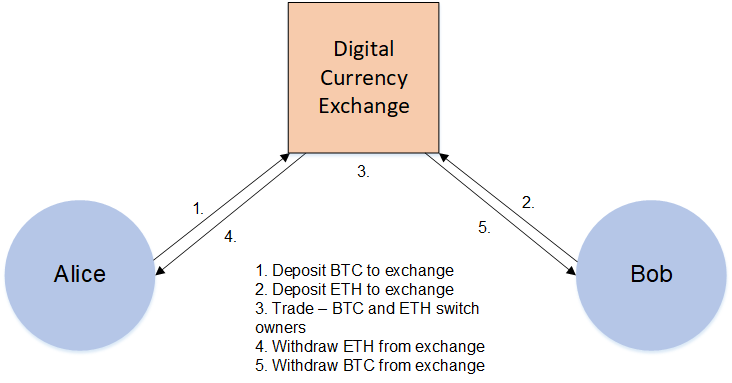
\includegraphics[width=.80\textwidth]{arch-ver-exch}
    \caption{Exchange of currencies using a third party -- a \acrfull{dcex}. The process begins by both Alice and Bobs depositing their respective currencies to the \acrshort{dcex}. \acrshort{dcex} then facilitates the trade of currencies and Alice and Bob can then withdraw their funds from the \acrshort{dcex}.}
    \label{fig:arch-ver-exch}
\end{figure}
% 
\subsection{Architecture}
% 
There are several possibilities, one wants to exchange cryptocurrency on the internet. Let's consider, that Alice wants to exchange Bitcoin for Ether. She would first find a cryptocurrency exchange that operates with both Bitcoin and Ether. She would probably need to create an account with that exchange and deposit her Bitcoins to that exchange's Bitcoin address. She could then trade the the Bitcoins for the Ether on the exchange's web-page with other registered users. Afterwards, she would withdraw the newly-acquired Ether from her exchange account to her private Ethereum wallet. This is more-less the standard procedure, \textbf{as we learned in the State of the Art.}

The issue with this approach is, that Alice needs to fully trust the exchange she chose. Exchange has full control over Alice's funds since she deposited the Bitcoins until she withdraws the Ether. In case that the exchange is attacked by hackers or is not protecting users' funds properly, Alice may never get her money back. The reputation of an exchange may provide little guidance on what exchange is trustworthy, but it is not a definite measure. In the aforementioned case of Mt. Gox, this was the most prominent exchange just weeks before its crash \cite{Popper2014ApparentTimes}.

An alternative approach for Alice could be, that she finds a person who wants to make an opposite trade to hers. Let's further assume, that Bob wants to exchange the same amount of currency from Ether to Bitcoin and that Alice can communicate with Bob by means other than the blockchains or cryptocurrency exchanges (e.g. a cryptocurrency forum). Alice and Bob need to agree on the amounts each of them is going to transfer and they need to exchange their public addresses - namely Alice needs to give Bob her Ethereum public address and Bob needs to give Alice his public Bitcoin address. Alice then sends her Bitcoins to Bob and Bob sends her Ether to Alice. This simple transaction is illustrated in figure \ref{fig:naive-approach}.

\begin{figure}[ht]
    \centering
    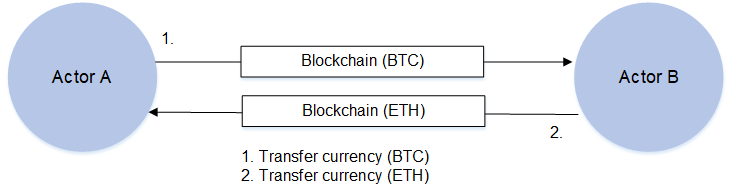
\includegraphics[width=.80\textwidth]{naive-approach}
    \caption{The naive approach to cryptocurrency exchange. Actor A (Alice) wants to buy Bitcoin (BTC) and Actor B (Bob) wants to buy Ether. }
    \label{fig:naive-approach}
\end{figure}

This removes the need to involve a third party in the transaction, but it does not completely solve the problem of trust. Since Alice and Bob might be located in different locations, it may be very difficult if not impossible, to ensure that the other party carries out the transaction as agreed. If Alice sends the funds to Bob, but Bob does not keep his side of the agreement and does not send his funds to Alice, it would be impossible for her to reverse the transaction. 

In an attempt to ensure that both keep their agreement, Alice and Bob could synchronise the moment when they send their transactions to the network. However, this does also not provide a fail-proof solution. For instance, Bob could subsequently send another transaction (transferring his funds to himself) from the same address, which could be processed by the network first, thus rendering the original transaction invalid.

\paragraph{Identification} 
If Alice did not receive the funds as agreed, she might want to involve traditional law-enforcement methods. But since the agreement happened over the internet, it may not be possible to successfully identify Bob.

When an reliable identification of an institution (such as an e-shop) is needed, the concept of public-key certificates has proven useful. The institution engages with a trusted third party, which then verifies the identity of this institution. Afterwards, the third party issues a certificate, that proves the identity of the institution to the visitors from the web, usually for a limited period of time \cite{Lee2013SecurityArchitects}. 

However, for a peer-to-peer relationship, digital certificates do not seem feasible, because the process of verification of someone's identity in real world is a lengthy process. We can now see the emerging need for a system, which does not require trusting a third party, nor trusting the trading partner. A decentralised system running on a blockchain might be the solution to this problem.

\paragraph{Black box architecture}
Let us introduce a `black box' between Alice and Bob. This box could hold funds from both parties and only release them under condition, that both Alice and Bob sent their respective amount. If one of them tried to cheat, the box would not release the funds further. The black box architecture is illustrated in figure \ref{fig:arch-ver0}.
% 
\begin{figure}[ht]
    \centering
    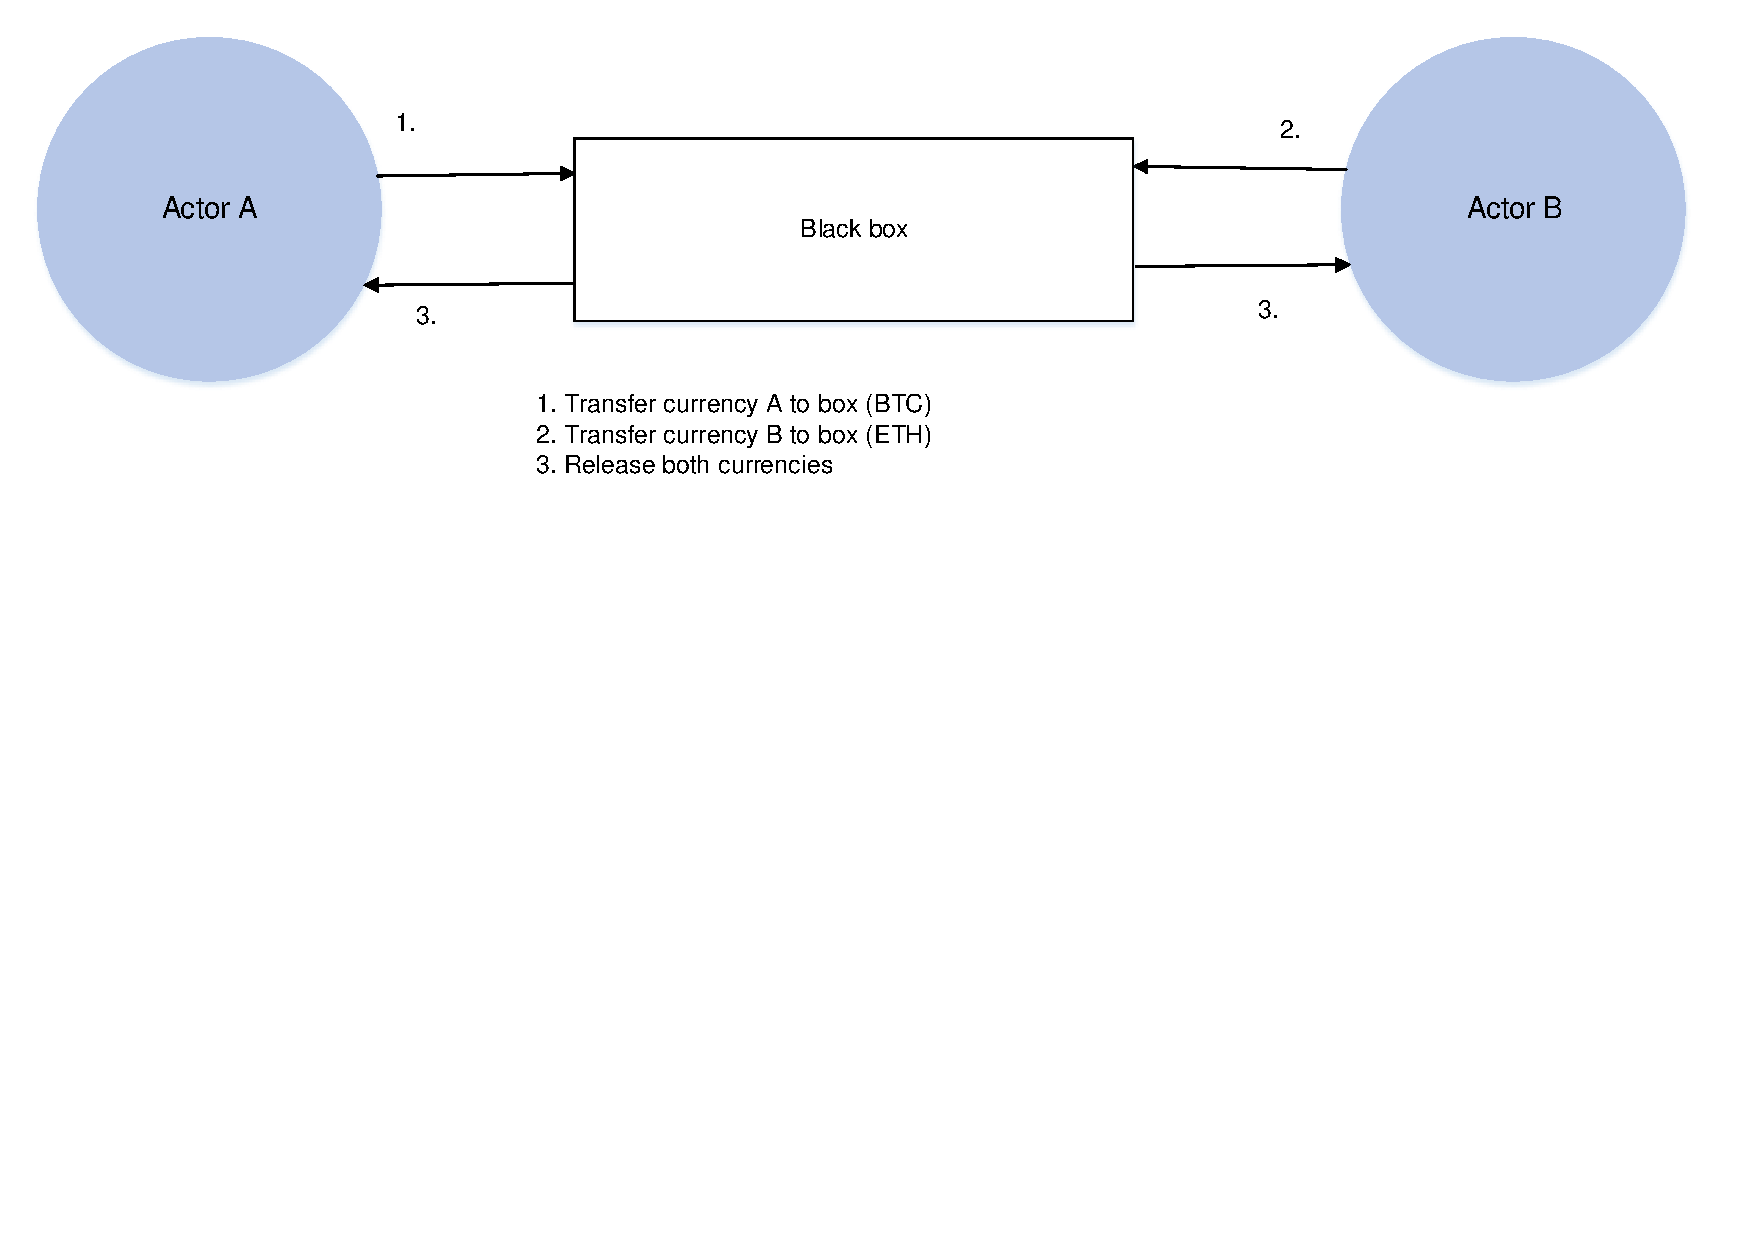
\includegraphics[width=.80\textwidth]{arch-ver0}
    \caption{Black box architecture. The black box spans both blockchains and only releases the funds, if it received the full amount from both parties.}
    \label{fig:arch-ver0}
\end{figure}

The black box is not a third party, rather an automated system that only operates with simple internal logic. This logic should be verifiable by anyone, however, it should not be possible to manipulate this logic by any of the parties. The black box would operate on top of both blockchains and would be decentralised. It would therefore fulfil our requirement for operation without a third party and without requiring the trading parties to trust each other.

This is a plausible architecture for a proposed system. It may be implemented on networks, that enable this kind of transaction control, either via multi-signature wallets (for example Bitcoin) or smart contracts (for example Ethereum). Another advantage is, that the parties now do not need to trust one another. In case of one party tries to cheat, the black box would not release the funds further.

The drawback of this architecture lies in technical complexity. The black box would need to operate on top of \textit{both} blockchains and would require coordination between two networks. The architecture could be simplified in order to remove the need to operate on two blockchains.

\paragraph{Black half-box architecture}
We can achieve similar functionality by only limiting the transaction control to one blockchain. This architecture could be referred to as `black half-box' and is illustrated in figure \ref{fig:half-box-arch}. In this scenario, after initial agreement has been made, Alice proceeds to send funds to the black half-box. This transaction is public and can be verified by Bob. When Bob sees, that the funds are deposited in the box, he can now transfer his funds to Alice. The black half-box queries the blockchain for Bob's transaction in regular intervals. Once the transaction has been successfully included in the blockchain, the black half-box recognises this and can now release Alice's funds to Bob.
% 
\begin{figure}[ht]
    \centering
    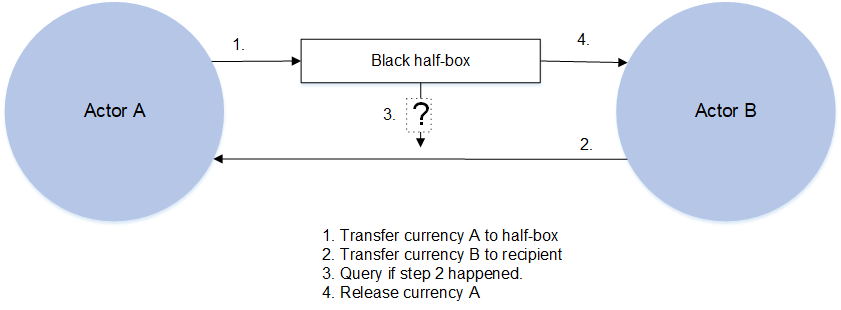
\includegraphics[width=.80\textwidth]{half-box-arch}
    \caption{Black half-box architecture. The box only controls funds on one of the blockchains. The transaction on the other blockchain happens normally. The box queries the blockchain for this transaction, and only releases the funds once it has been processed.}
    \label{fig:half-box-arch}
\end{figure}

This architecture solves the technical drawbacks of the regular black box. However, it can only work safely, if the sequence of steps is followed. In case the funds from Bob to Alice were sent \textit{before} Alice deposited her part in the half-box, Alice is not bound to keep her part of the agreement.

Currently, this architecture could be implemented in two ways: utilising multi-signature wallets

//Write about multi-sig wallet possibilities - 1-way-sig, 2-way-sig, 3-way-sig

//Write about use with Smart contacts, then present the tech-version of the diagram above.






% Regular transactions made in the Bitcoin, Ethereum, Litecoin or other coins are irreversible and once they are processed by the network, they cannot be changed. But what if a condition could be included in the transaction? A `black box' that collects funds 


% that only Some systems (Bitcoin, Ethereum) provide a functionality known as multi-signature wallets



\begin{figure}[ht]
    \centering
    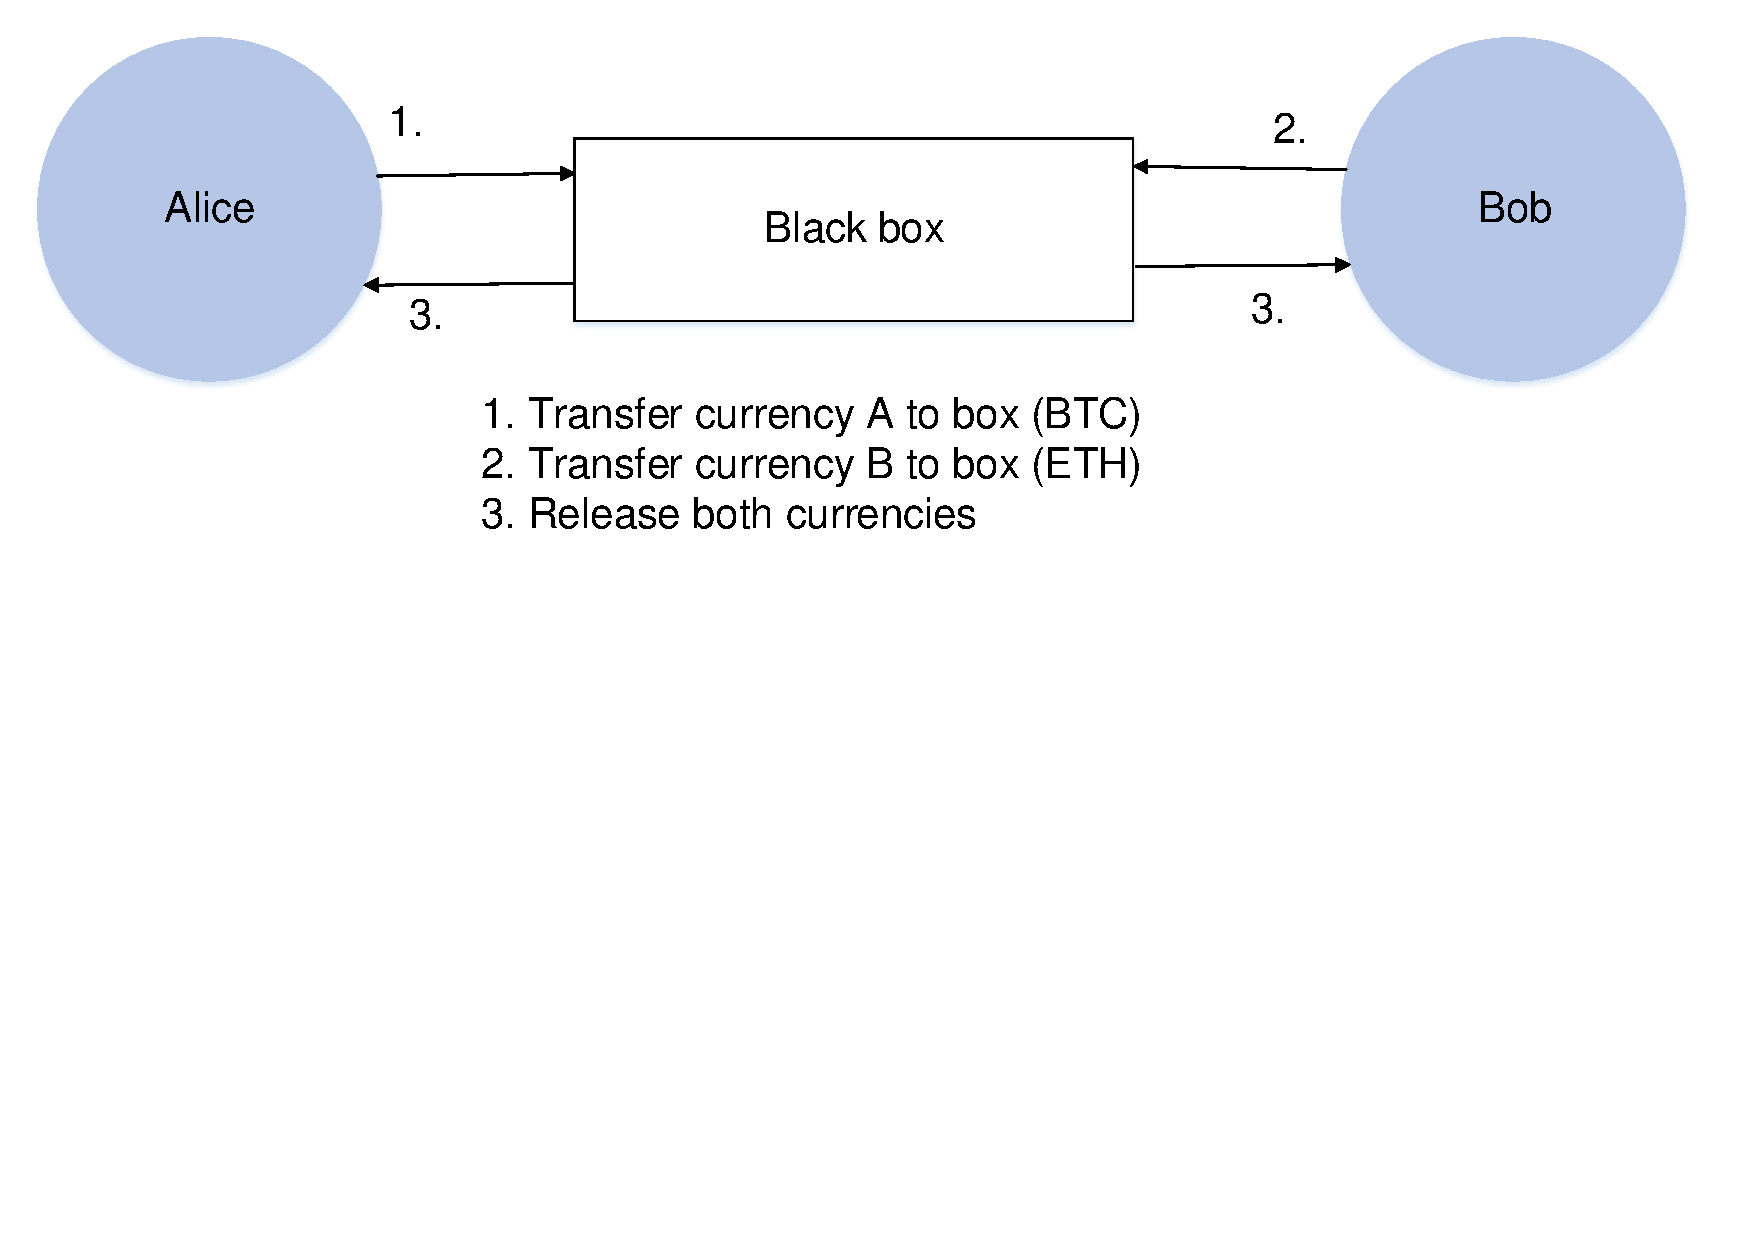
\includegraphics[width=.80\textwidth]{arch-ver1}
    \caption{}
    \label{fig:arch-ver1}
\end{figure}
